% Basic stuff
\documentclass[a4paper,10pt]{article}
\usepackage[nswissgerman]{babel}
\usepackage{scrextend}

% 3 column landscape layout with fewer margins
\usepackage[landscape, left=0.75cm, top=1cm, right=0.75cm, bottom=1.5cm, footskip=15pt]{geometry}
\usepackage{flowfram}
\ffvadjustfalse
\setlength{\columnsep}{1cm}
\Ncolumn[<10]{3}
\onecolumn[10]

% define nice looking boxes
\usepackage[many]{tcolorbox}
\changefontsizes[9pt]{9pt}

% a base set, that is then customised
\tcbset {
	base/.style={
		boxrule=0mm,
		leftrule=1mm,
		left=1.75mm,
		arc=0mm, 
		fonttitle=\bfseries, 
		colbacktitle=black!10!white, 
		coltitle=black, 
		toptitle=0.75mm, 
		bottomtitle=0.25mm,
		title={#1}
	}
}

\definecolor{brandblue}{rgb}{0.34, 0.7, 1}
\newtcolorbox{mainbox}[1]{
	colframe=brandblue, 
	base={#1}
}

\newtcolorbox{subbox}[1]{
	colframe=black!20!white,
	base={#1}
}

% Mathematical typesetting & symbols
\usepackage{amsthm, mathtools, amssymb} 
\usepackage{marvosym, wasysym}
\allowdisplaybreaks

% Tables
\usepackage{tabularx, multirow}
\usepackage{makecell}
\usepackage{booktabs}
\renewcommand*{\arraystretch}{2}

% Make enumerations more compact
\usepackage{enumitem}
\setitemize{itemsep=0.5pt}
\setenumerate{itemsep=0.75pt}

% To include sketches & PDFs
\usepackage{graphicx}

% For hyperlinks
\usepackage{hyperref}
\hypersetup{
	colorlinks=true
}

% Metadata
\title{Cheatsheet\\ Wahrscheinlichkeit \& Statistik}
\author{Julian Steinmann}
\date{\vspace{-10pt}Sommer 2022}

% Math helper stuff
\def\limxo{\lim_{x\to 0}}
\def\limxi{\lim_{x\to\infty}}
\def\limxn{\lim_{x\to-\infty}}
\def\R{\mathbb{R}}
\def\P{\mathbb{P}}
\def\F{\mathcal{F}}
\def\sumn{\sum_{n=0}^\infty}
\def\sumk{\sum_{k=1}^\infty}
\def\E{\mathbb{E}}
\DeclareMathOperator{\Var}{\text{Var}}
\newcommand{\middot}{~\textperiodcentered~}
\newlist{rowlist}{enumerate*}{1}
\setlist[rowlist]{label={\textbf{\roman*}\text{: }}, afterlabel={}, itemjoin=\middot}


\begin{document}


\begin{center}
    Lizenziert unter CC BY-SA 4.0. Für Urheber, Quellen und Lizenzinformationen, siehe:\\
    \href{https://github.com/thomasgassmann/eth-cheatsheets}{github.com/thomasgassmann/eth-cheatsheets}

    GITCOMMIT
\end{center}


Dieses Cheatsheet basiert auf dem \href{https://github.com/XYQuadrat/eth-cheatsheets}{WuS Cheatsheet von xyquadrat}.

\section{Grundbegriffe}
\begin{subbox}{Definition Wahrscheinlichkeitraum}
	Ein Wahrscheinlichkeitraum ist ein Tupel \((\Omega, \F, \P)\):
	\begin{itemize}
		\item Die Menge \(\Omega\) nenen wir \textbf{Grundraum}. Ein \(\omega \in \Omega\) nennen wir Elementarereignis.
		\item \(\F \subseteq \mathcal{P}(\Omega)\) ist eine \textbf{Sigma-Algebra}.
		\item \(\P\) ist ein \textbf{Wahrscheinlichkeitsmass} definiert auf \((\Omega, \F)\).
	\end{itemize}
	Dabei ist \(A \subseteq \Omega\) ein Ereignis.
\end{subbox}

\subsection{Sigma-Algebra}
Eine Sigma-Algebra ist ein Subset \(\F \subseteq \mathcal{P}(\Omega)\) mit den folgenden Eigenschaften:
\begin{enumerate}
	\item \(\Omega \in \F\)
	\item \(A \in \F \implies A^\complement \in \F\)
	\item \(A_1, A_2, \ldots \in \F \implies \bigcup_{i=1}^\infty A_i \in \F\)
	\item \(\varnothing \in \F\)
	\item \(A_1, A_2, \ldots \in \F \implies \bigcap_{i=1}^\infty A_i \in \F\)
	\item \(A, B \in \F \implies A \cup B \in \F\)
	\item \(A, B \in \F \implies A \cap B \in \F\)
\end{enumerate}
Die ersten drei Punkte sind dabei gerade die Definition einer Sigma-Algebra.

Nützlich ist ausserdem die De-Morgan-Regel: \[(\cup_{i=1}^\infty A_i)^\complement = \cap_{i=1}^\infty(A_i)^\complement\]

\subsection{Wahrscheinlichkeitsmass}
Ein Wahrscheinlichkeitsmass \(\P\) ist eine Abbildung
\begin{align*}
	\P: \  & \F \mapsto \left[0,1\right] \\
	       & A \mapsto \P[A]
\end{align*}
mit den Eigenschaften
\begin{enumerate}
	\item \(\P[\Omega] = 1\)
	\item \(\P [A] = \sum_{i=1}^\infty P[A_i]\), falls \(A = \bigsqcup_{i=1}^\infty A_i\)
	\item \(\P[\varnothing] = 0\)
	\item \(\P[A^\complement] = 1 - \P[A]\)
	\item \(\P[A \cup B] = \P[A] + P[B] - \P[A\cap B]\)
	\item \(A \subseteq B \implies \P[A] \le \P[B]\) (Monotonie)
	\item \(\P[\bigcup_{i=1}^\infty A_i] \le \sum_{i=1}^\infty \P[A_i]\) (Union Bound)
\end{enumerate}

Wenn \(A_1, \ldots A_n\) paarweise disjunkt sind, gilt:
\[\P[A_1 \cup \ldots \cup A_n] = \P[A_1] + \ldots + \P[A_n]\]

Ausserdem gilt (Prinzip der Inklusion/Exklusion):

$$
	\P \left[ \bigcup_{i=1}^n A_i \right] = \sum_{l=1}^n (-1)^{l+1} \left( \sum_{1 \leq i_1 < \cdots < i_l \leq n} \P \left[ A_{i_1} \cap \cdots \cap A_{i_l} \right] \right)
$$

\subsection{Bedingte Wahrscheinlichkeiten}
Sei \((\Omega, \F, \P)\) ein Wahrscheinlichkeitsraum mit \(A, B \in \F\) und \(\P[B] > 0\). Die bedingte Wahrscheinlichkeit von \(A\) gegeben \(B\) ist definiert als:
\[\P[A|B] = \frac{\P[A\cap B]}{\P[B]}\]
\begin{subbox}{Totale Wahrscheinlichkeit}
	Sei \(B_1, \ldots, B_n \in \F\) eine Partition von \(\Omega\) mit \(\P[B_i] > 0\) für alle \(1 \le i \le n\). Dann gilt:
	\[\forall A \in \F \quad \P[A] = \sum_{i=1}^{n} \P[A|B_i] \ \P[B_i]\]
\end{subbox}
\begin{mainbox}{Satz von Bayes}
	Sei \(B_1, \ldots, B_n \in \F\) eine Partition von \(\Omega\) mit \(\P[B_i] > 0\) für jedes \(i\). Für jeden Event \(A\) mit \(\P[A] > 0\) gilt:
	\[\forall i = 1,\ldots, n \quad \P[B_i|A] = \frac{\P[A|B_i] \ \P[B_i]}{\sum_{k=1}^n \P[A|B_k] \ \P[B_k]}\]
\end{mainbox}

Wir definieren den bedingten Erwartungswert:

$$
	\E[X \mid B] = \frac{\E[1_B X]}{\P[B]} = \sum_{x \in X(\Omega)} x \P[X = x \mid B]
$$

Für eine Partition $\mathcal{B} = (B_i)_{i \in I}$ von $\Omega$ definieren wir:

$$
	\E[X \mid \mathcal{B}](\omega) = \sum_{i \in I, \P[B_i] > 0} \E[X \mid B_i] 1_{B_i}(\omega)
$$

Ähnlich definieren wir auch die bedingte Dichte:

$$
	f_{X \mid Y}(x \mid y) = \frac{f_{X,Y}(x,y)}{f_Y(y)}
$$

\subsection{Unabhängigkeit}
\begin{mainbox}{Definition Unabhängigkeit}
	Zwei Ereignisse \(A, B\in \F\) sind unabhängig, falls gilt:
	\[\P[A\cap B] = \P[A] \cdot \P[B]\]
	Alternative Definitionen sind:
	\[\P[A|B] = \P[A] \text{ bzw. } \P[B|A] = \P[B]\]
\end{mainbox}
\begin{itemize}
	\item Falls \(\P[A] \in \{0,1\}\), dann ist \(A\) zu jedem Ereignis unabhängig.
	\item Wenn ein Ereignis \(A\) unabhängig zu sich selbst ist, dann folgt \(\P[A] \in \{0,1\}\).
	\item Wenn \(A, B\) unabhängig sind, dann sind auch \(A, B^\complement\) unabhängig.
\end{itemize}
\subsubsection*{Unabhängigkeit für mehrere Ereignisse}
Seien \(A_1, \ldots, A_n \in F\), dann sind die Ereignisse unabhängig, falls gilt:
\[\forall I \subseteq \{1, \ldots, n\} \quad \P \left[ \bigcap_{i\in I}A_i \right] = \prod_{i\in I} \P[A_i]\]

\section{Zufallsvariablen}
Eine Zufallsvariable ist eine Abbildung \(X: \Omega \mapsto \R\) mit
\[\forall x \in \R \quad \{\omega \in \Omega \mid X(\omega) \leq x\} \in \F\]
Dabei lassen wir das \(\omega\) oft weg und schreiben nur \(X\).

\subsection{Verteilungsfunktion}
\begin{mainbox}{Definition Verteilungsfunktion}
	Die Verteilungsfunktion ist die Abbildung \(F_X: \ \R \mapsto [0,1]\) definiert durch
	\[\forall x \in \R \quad F_X(x) = \P[X \le x]\]
\end{mainbox}
Die Verteilungsfunktion hat folgende Eigenschaften:
\begin{enumerate}
	\item \(a < b \implies \P[a < X \le b] = F_X(b) - F_X(a)\)
	\item \(F\) ist monoton wachsend
	\item \(F\) ist rechtsstetig, d.h. \(\lim_{t \to 0} F_{x+t} = F(x)\)
	\item \(\lim_{x\to - \infty} F_X(x) = 0\) und \(\lim_{x\to \infty} F_X(x) = 1\)
\end{enumerate}

Sind die letzten drei Punkte erfüllt existiert auch eine Zufallsvariable mit der entsprechenden Verteilungsfunktion.

\subsubsection*{Linksstetigkeit}
Die Definition der Linksstetigkeit ist
\[F(x-) = \lim_{t\to 0} F(x-t)\]
Es gilt allerdings \textit{nicht} immer \(F(x-) = F(x)\), d.h. nicht jede Verteilungsfunktion ist linksstetig. Allerdings gilt:
\[\forall x \in \R \quad F(x) - F(x-) = \P[X=x]\]
Daraus lässt sich für stetige ZV \(P[X=x] = 0\) folgern.\\
Ausserdem gilt für eine monoton steigende Folge $(A_n)$ von Mengen ($A_n \subseteq A_{n+1}$) dass $\lim_{n \to \infty} \P[A_n] = \P[\bigcup_{n=1}^\infty A_n]$.\\
Gleichermassen für eine monoton fallende Folge $(A_n)$ ($A_{n+1} \subseteq A_n$) dass $\lim_{n \to \infty} \P[A_n] = \P[\bigcap_{n=1}^\infty A_n]$.

\subsection{Unabhängigkeit}
Die Zufallsvariablen \(X_1, \ldots, X_n\) sind unabhängig, falls:
\begin{align*}
	\forall x_1, \ldots, x_n \in \R: \quad & \P[X_1 \le x_1, \ldots, X_n \le x_n] =             \\
	                                       & \P[X_1 \le x_1] \cdot \ldots \cdot \P[X_n \le x_n]
\end{align*}
Eine Folge von Zufallsvariablen \(X_1, X_2, \ldots\) ist unabhängig, falls \(
\forall n \ X_1, \ldots X_n\) unabhängig sind. Sie ist zusätzlich identisch verteilt (uiv.), falls ausserdem \(\forall i,j \quad F_{X_i} = F_{X_j}\) gilt.

\subsection{Transformationssatz}

\begin{mainbox}{}
	Sei $X = (X_1, \cdots, X_n)^\top$ eine Zufallsvariable in $\R^n$ und Dichtefunktion $f_X: \R^n \mapsto \R_+$. Sei $Y := \phi(X)$ mit $\phi: \R^n \mapsto \R^n$ invertierbar. Dann gilt:
	$$f_Y(y) = f_X(\phi^{-1}(y)) \left| \det \left( J_{\phi^{-1}}(y) \right) \right|$$
\end{mainbox}

\begin{mainbox}{Linearer Fall}
	Falls $X$ $n$-dimensional stetig und $g: \R^n \mapsto \R^n$ linear mit $g(t) = m + Bt$ ist ($\det(B) \neq 0$) erhalten wir:
	$$
		f_Y(t) = \frac{1}{\left| \det \left( B \right) \right|} f_X \left( B^{-1} (t - m) \right)
	$$
	wobei $Y = g(X)$.
\end{mainbox}

\subsection{Konstruktion einer Zufallsvariable}
Gegeben eine Verteilungsfunktion \(F_X\) wollen wir die entsprechende ZV \(X\) konstruieren.
\begin{subbox}{Kolmogorov-Theorem}
	Es existiert \((\Omega, \F,\P)\) und ZVs \( X_1, X_2, \ldots\), sodass \(X_1, X_2, \ldots\) uiv. Bernoullivariablen mit \(p = 0.5\) sind.
\end{subbox}

Sei \(X_1, X_2,\ldots \sim \text{Ber}(1/2)\) eine unendliche Folge, dann ist
\[U = \sum_{n = 1}^\infty 2^{-n}\cdot X_n\]
gleichverteilt auf \([0,1]\).

Aufgrund der Eigenschaften der Verteilungsfunktion \(F\) wissen wir, dass eine eindeutige Inverse $F^{-1}$ existiert. Wir können die generalisierte Inverse definieren als: \[\forall \alpha \in [0,1] \quad F^{-1}(\alpha) = \inf \{x \in \R \mid F(x) \geq \alpha\}\]

Sei nun \(F\) eine Verteilungsfunktion und \(U\) eine gleichverteilte ZV in \([0,1]\). Dann besitzt \(X = F^{-1}(U)\) genau die Verteilungsfunktion \(F_X = F\).

\begin{subbox}{Fast sichere Ereignisse}
	Ein Ereignis \(A \in \F\) tritt fast sicher (f.s) ein, falls \(\P[A] = 1\). Seien \(X, Y\) ZV, so schreiben wir \(X \le Y \text{ f.s.} \iff \P[X\le Y] = 1\).
\end{subbox}

\subsection{Diskrete Zufallsvariablen}
\begin{subbox}{Definition diskrete ZV}
	Eine ZV \(X\) heisst diskret, falls \(\exists W \subset \R\) endlich oder abzählbar, so dass \(X \in W\) f.s. Falls \(\Omega\) endlich oder abzählbar ist, dann ist \(X\) immer diskret.
\end{subbox}
\noindent Die Verteilungsfunktion einer diskreten ZV ist:
\[(p(x))_{x \in W} \text{ wobei } \sum_{x\in W} p(x) = 1\]
Die Gewichtsfunktion einer diskreten ZV ist:
\[\forall x \in W \quad p(x) = \P[X=x]\]

\subsection{Diskrete Verteilungen}
\textbf{Bernoulli-Verteilung} (\(X \sim \text{Ber}(p)\)): Hat nur die Ereignisse \(\{0,1\}\). Sie ist definiert als
\[\P[X=0] = 1-p \text{ und } \P[X=1]=p\]

\noindent \textbf{Binomialverteilung} (\(X \sim \text{Bin}(n,p)\)): Die Wiederholung von Bernoulli-Experimenten. Sie ist definiert als
\[\forall k \in \{0, \ldots, n\} \quad \P[X=k] = \binom{n}{k} \cdot p^k \cdot (1-p)^{n-k}\]

\noindent \textbf{Geometrische Verteilung} (\(X \sim \text{Geom}(p)\)): Beschreibt das erste Auftreten eines Erfolges. Sie ist definiert als
\[\forall k \in \mathbb{N} - \{0\} \quad \P[X=k]=(1-p)^{k-1}\cdot p\]

\noindent \textbf{Poisson-Verteilung} (\(X \sim \text{Poisson}(\lambda)\)): Annäherung an die Binomialverteilung für grosse \(n\) und kleine \(p\) (d.h. rare Ereignisse). Sie ist definiert als
\[\forall k \in \mathbb{N}, \lambda > 0 \quad \P[X=k]=\frac{\lambda^k}{k!}\cdot e^{-\lambda}\]

Für $X_n \sim \text{Bin}(n, p_n)$ mit $n p_n = \lambda$ gilt $\lim_{n \to \infty} \P[X_n = k] = \P[X = k]$ wobei $X \sim \text{Poisson}(\lambda)$.

Ausserdem gilt für $X \sim P(\lambda), Y \sim P(\mu)$ dass $X + Y \sim P(\lambda + \mu)$.


\subsection{Stetige Zufallsvariablen}
\begin{subbox}{Definition stetige ZV}
	Eine ZV \(X\) heisst stetig, wenn ihre Verteilungsfunktion \(F_X\) wie folgt geschrieben werden kann:
	\[\forall x \in \R \quad F_X(x) = \int_{-\infty}^x f(y) \mathop{dy}\]
\end{subbox}
Hierbei ist \(f: \R \mapsto \R_+\) die Dichte von X. Für die Dichte gilt:
\[\int_{-\infty}^{+\infty}f(y) \mathop{dy} = 1\]
Es gelten folgende Eigenschaften:
\begin{enumerate}
	\item \(\P[a \le x \le b] = \P[a < x < b]\)
	\item \(\P[X=x] = 0\)
	\item \(\P[X \in [a,b]] = \P[X \in (a,b)]\)
\end{enumerate}

\subsection{Stetige Verteilungen}
\textbf{Gleichverteilung} (\(X \sim \mathcal{U}[a,b]\)): Jedes Ereignis hat die gleiche Wahrscheinlichkeit. Sie ist definiert als
\[f_{a,b}(x) = \begin{cases}
		0             & x \notin [a,b] \\
		\frac{1}{b-a} & x \in [a,b]
	\end{cases}\]

\noindent \textbf{Exponentialverteilung} (\(X \sim \text{Exp}(\lambda)\)): Das stetige Gegenstück zur Geometrischen Verteilung. Sie ist definiert als
\[f_{a,b}(x) = \begin{cases}
		0                            & x < 0    \\
		\lambda \cdot e^{-\lambda x} & x \geq 0
	\end{cases}\]
\begin{itemize}
	\item Wenn \(Y\sim \text{Exp}(\lambda)\), dann ist \(c \cdot Y \sim \text{Exp}(\frac{\lambda}{c})\)
	\item \(X_1, X_2 \sim \mathcal{N}(0,1)\) uiv. \(\implies \chi_2 = X_1^2 +X_2^2 \sim \text{Exp}(\frac{1}{2})\)
	\item Die Summe von $n$ exponentialverteilten ZV mit 
\end{itemize}

\noindent \textbf{Normalverteilung} (\(X \sim \mathcal{N}(m, \sigma^2)\)): Die wohl wichtigste Verteilung. Sie ist definiert als
\[f_{m, \sigma}(x) = \frac{1}{\sqrt{2 \pi \sigma^2}} \cdot e^{-\frac{(x-m)^2}{2 \sigma^2}}\]

\(X \sim \mathcal{N}(0,1)\) wird auch Standardnormalverteilung genannt. Für eine standardnormalverteilte ZV \(X\) gilt
\[Z = m +\sigma \cdot X \sim \mathcal{N}(m, \sigma^2)\]

Die Summe von uiv. normalverteilten Zufallsvariablen ist auch normalverteilt.

\section{Erwartungswert}
\begin{mainbox}{Definition Erwartungswert}
	Sei \(X: \Omega \mapsto \R_+\) eine ZV mit nicht-negativen Werten. Dann ist
	\[\E[X] = \int_0^\infty 1- F_X(x) \mathop{dx}\]
	der Erwartungswert von \(X\).
\end{mainbox}
Wenn \(\E[|X|] < \infty\), dann ist der Erwartungswert definiert als
\[\E[X] = \E[X_+] - \E[X_-]\]

\subsection{Erwartungswert diskreter ZV}
Sei \(X\) eine diskrete ZV mit \(X \in W\) f.s. Sei \(\phi: \R \mapsto \R\) eine Abbildung. Falls die Summe absolut konvergiert, gilt
\[\E[\phi(X)] = \sum_{x\in W} \phi(x)\cdot \P[X=x]\]
Sei \(\phi = \) id, gilt
\[
	\E[X] = \sum_{x\in W} x \cdot \P[X=x]
	.\]

\subsection{Erwartungswert stetiger ZV}
Sei \(X\) eine stetige ZV mit Dichtefunktion \(f\). Sei \(\phi :\R\mapsto \R\) eine Abbildung, sodass \(\phi(x)\) eine Zufallsvariable ist. Sofern das Integral absolut konvergiert ist, gilt
\[\E[\phi(X)] = \int_{-\infty}^{\infty}\phi(x)f(x) \mathop{dx}\]
Die Definition für \(\phi = \) id ist analog zum diskreten Fall.
\subsubsection{\texorpdfstring{Bestimmen der Dichte von \(f(X)\)}{Bestimmen der Dichte von f(X)}}
\begin{enumerate}
	\item Sei \(\phi: \R \mapsto \R\) stückweise beschränkt und stetig.
	\item \(\E[\phi(Y)] = \E[\phi(f(X))] = \E[\tau(X)]\)
	\item Dichte von \(X\) in vorheriger Gleichung einsetzen.
	\item Variablenwechsel \(u = f(x)\) \& Grenzen anpassen
\end{enumerate}

\subsection{Rechnen mit Erwartungswerten}
\begin{subbox}{Linearität des Erwartungswertes}
	Seien \(X,Z\) ZV mit \(\lambda \in \R\). Falls die Erwartungswerte wohldefiniert sind, gilt
	\begin{align*}
		\E[\lambda \cdot X] & = \lambda \cdot \E[X] \\
		\E[X + Y]           & = \E[X] + \E[Y]       \\
	\end{align*}
\end{subbox}
Falls zwei ZV \(X,Y\) unabhängig sind, gilt auch
\[\E[X\cdot Y] = \E[X] \cdot \E[Y]\]

Für Divison hingegen gilt:
\[\E[\frac{X}{Y}] = \E[X] \cdot \E[\frac{1}{Y}]\]

\begin{subbox}{Alternativdefinition unabhängige ZV}
	Seien \(X_1, \ldots, X_n\) diskrete ZV. Dann sind folgende Aussagen äquivalent:
	\begin{enumerate}
		\item \(X_1, \ldots, X_n\) sind unabhängig.
		\item Für jedes \(\phi_1, \ldots, \phi_n: \R \mapsto\R\) beschränkt gilt:
	\end{enumerate}
	\[\E[\phi_1(X_1)\cdot\ldots\cdot\phi_n(X_n)] = \E[\phi_1(X_1)] \cdot\ldots\cdot \E[\phi_n(X_n)]\]
\end{subbox}

\subsection{Extremwertformel}
Sei \(X\) eine diskrete ZV mit Werten in \(\mathbb{N}\). Dann gilt folgende Identität:
\[\E[X] = \sum_{n=1}^\infty \P[X\ge n]\]
Sei \(X\) eine stetige ZV mit \(X \ge 0\) f.s., dann gilt:
\[\E[X] = \int_0^\infty \P[X > x] \mathop{dx}\]

\subsection{Momentenerzeugende Funktion}

\begin{subbox}{Momentenerzeugende Funktion}
	Sei $X$ eine Zufallsvariable. Die momentenerzeugende Funktion ist definiert als:
	$$
		M_X(t) := \E \left[ e^{tX} \right]
	$$
\end{subbox}

\subsection{Ungleichungen}
\begin{subbox}{Monotonie}
	Seien \(X, Y\) ZV sodass \(X \le Y\) f.s., dann gilt \(\E[X] \le \E[Y]\).
\end{subbox}

\begin{subbox}{Jensen-Ungleichung}
	Sei \(X\) eine ZV und \(\phi : \R \mapsto \R\) eine konvexe Funktion, dann gilt:
	\[\phi(\E[X]) \le \E[\phi(X)]\]
\end{subbox}

\begin{mainbox}{Markov-Ungleichung}
	Sei \(X\) eine ZV mit \(X \ge 0\) f.s., dann gilt für jedes \(a > 0\):
	\[\P[X\ge a] \le \frac{\E[X]}{a}\]
	Allgemeiner für eine beliebige Zufallsvariable $X$ und eine wachsende Funktion $g: \mathcal{W}(X) \mapsto [0, \infty)$ für jedes $c \in \R$ mit $g(c) > 0$ dass:
	$$\P[X \geq c] \leq \frac{\E[g(X)]}{g(c)}$$
\end{mainbox}

\subsection{Varianz}
Sei \(X\) eine ZV sodass \(\E[X^2] < \infty\). Die Varianz von \(X\) ist definiert durch
\[\Var[X] = \sigma_X^2 = \E[(X-m)^2]\]
wobei \(m=\E[X]\). Dabei wird \(\sigma_X\) auch die Standardabweichung von \(X\) genannt und beschreibt die typische Distanz eines Wertes \(x\in X\) zu \(\E[X]\).

\begin{subbox}{Chebychev-Ungleichung}
	Wenn \(X\) eine ZV mit \(\E[X^2] < \infty\) ist, dann gilt für jedes \(a \ge 0\):
	\[\P[|X - \E[X]| \ge a] \le \frac{\Var[X]}{a^2}\]
\end{subbox}

\begin{enumerate}
	\item Wenn \(\E[X^2] < \infty\), dann \(\Var[X] = \E[X^2] - \E[X]^2\).
	\item Wenn \(\E[X^2] < \infty\) und \(a, b \in \R\), dann \(\Var[a X + b] = a^2 \Var[X]\).
	\item Wenn \(S = X_1 + \ldots + X_n\), wobei \(X_1, \ldots, X_n\) paarweise unabhängig sind, dann gilt \(\sigma_S^2 = \sigma_{X_1}^2 + \ldots + \sigma_{X_n}^2\).
\end{enumerate}

\subsection{Kovarianz}
Wir können mit der Kovarianz die Abhängigkeit von zwei Zufallsvariablen messen.
\begin{subbox}{Definition Kovarianz}
	Wenn \(X, Y\) zwei ZV mit \(\E[X^2] < \infty, \E[Y^2] < \infty\), dann ist die Kovarianz zwischen \(X, Y\) definiert als
	\[\text{Cov}(X,Y) = \E[X \cdot Y] - \E[X] \cdot \E[Y]\]
	Falls $\text{Cov}(X,Y) = 0$ nennt man $X, Y$ unkorreliert.
\end{subbox}
\begin{itemize}
	\item \(\text{Cov}(X,X) = \sigma_X^2\)
	\item X, Y unabhängig \(\implies \text{Cov}(X,Y) = 0\)
\end{itemize}

\section{Gemeinsame Verteilungen}
\subsection{Diskrete gemeinsame Verteilungen}
\begin{subbox}{Definition gemeinsame Verteilung}
	Seien \(X_1, \ldots, X_n\) diskrete Zufallsvariablen wobei \(X_i \in W_i\) f.s. für \(W_i \subset \R\). Die gemeinsame Verteilung (GV) von \(X_1, \ldots, X_n\) ist die Familie \(p = (p(x_1, \ldots, x_n))_{x_1 \in W_1, \ldots, x_n \in W_n}\) definiert durch
	\[p(x_1, \ldots, x_n) = \P[X_1 = x_1, \ldots, X_n = x_n]\]
\end{subbox}

Seien \(X_1,\ldots,X_n\) diskrete ZV mit \(X_i \in W_i\) f.s. für \(W_i \subset \R\) und \(\phi: \R^n \mapsto \R\), so ist \(Z = \phi(X_1, \ldots, X_n)\) eine diskrete ZV mit Werten in \(W = \phi(W_1 \times \ldots \times W_n)\) und folgender Verteilung:
\[\forall z \in W. \ \P[Z = z] = \sum_{\substack{\phi(x_1, \ldots, x_n) \\= z}} \P[X_1 = x_1, \ldots, X_n = x_n]\]

Seien \(X_1,\ldots,X_n\) diskrete ZV mit \(X_i \in W_i\) f.s. mit GV \(p\). Dann ist die Randverteilung \(\forall z \in W_i\):
\[\P[X_i = z] = \sum_{\substack{x_1, \ldots, x_{i-1}, \\x_{i+1},\ldots,x_n}} p(x_1, \ldots, x_{i-1}, z, x_{i+1},\ldots,x_n)\]

Seien \(X_1,\ldots,X_n\) diskrete ZV mit GV \(p\) und \(\phi : \R^n \mapsto \R\). Dann ist der Erwartungswert definiert als:
\[\E[\phi(X_1, \ldots, X_n)] = \sum_{x_1,\ldots,x_n} \phi(x_1,\ldots,x_n) \cdot p(x_1,\ldots,x_n)\]

Seien \(X_1,\ldots,X_n\) diskrete ZV mit GV \(p\), dann sind die folgenden Aussagen äquivalent:
\begin{enumerate}
	\item \(X_1,\ldots,X_n\) sind unabhängig
	\item Für alle \(x_1 \in W_1, \ldots, x_n \in W_n\) gilt:
	      \(p(x_1,\ldots,x_n) = \P[X_1 = x_1] \cdot \ldots \cdot \P[X_n = x_n]\)
\end{enumerate}

Die gemeinsame Verteilung von \(X_1, \ldots, X_n\) erfüllt
\[\sum_{x_1\in W_1, \ldots, x_n \in W_n} p(x_1, \ldots, x_n) = 1\]

\subsection{Stetige gemeinsame Verteilungen}
\begin{subbox}{Definition gemeinsame Verteilung}
	Seien \(X_1, \ldots, X_n\) stetige ZV, so haben sie eine gemeinsame Verteilung, falls eine Funktion \(f: \R^n \mapsto \R_+\) existiert, die für jedes \(a_1, \ldots, a_n \in \R\) folgende Eigenschaft erfüllt:
	\begin{align*}
		\P[X_1 \le a_1, \ldots, X_n \le a_n] \\= \int_{-\infty}^{a_1} \cdots \int_{-\infty}^{a_n} f(x_1, \ldots, x_n) \mathop{dx_n} \ldots \mathop{dx_1}
	\end{align*}
	Dann ist \(f\) die \textbf{gemeinsame Dichte}.
\end{subbox}

Seien \(X_1, \ldots, X_n\) stetige ZV mit einer gemeinsamen Dichte \(f\) und \(\phi: \R^n \mapsto \R\). Dann ist der Erwartungswert definiert als
\begin{align*}
	\E[\phi(X_1, \ldots, X_n)] \\= \int_{-\infty}^\infty \cdots \int_{-\infty}^\infty \phi(x_1, \ldots, x_n) f(x_1, \ldots, x_n) \mathop{dx_n} \ldots \mathop{dx_1}
\end{align*}

Falls \(X_1, \ldots, X_n\) eine gemeinsame Dichte \(f\) besitzen, ist die Randverteilung
\begin{align*}
	f_i(z) = \int_{x_1, \ldots, x_{i-1}, x_{i+1}, \ldots, x_n \in \R^{n-1}}               \\
	f(x_1, \ldots, x_{i-1}, z, x_{i+1}, \ldots, x_n) \mathop{dx_n} \ \ldots \mathop{dx_1} \\
\end{align*}

Wenn \(X_1, \ldots, X_n\) stetige ZV mit Dichten \(f_1, \ldots, f_n\) sind, dann sind die folgenden Aussagen äquivalent:
\begin{enumerate}
	\item \(X_1, \ldots, X_n\) sind unabhängig
	\item \(X_1, \ldots, X_n\) sind stetig mit gemeinsamer Dichte
	      \[f(x_1, \ldots, x_n) = f_1(x_1) \cdot \ldots \cdot f_n(x_n)\]
	\item Für alle \(\phi_1, \ldots, \phi_n: \R \mapsto \R\) gilt:
	      \[\E[\phi_1 (x_1)\cdot \ldots\cdot (x_n)] = \E[\phi_1(x_1)] \cdot \ldots \cdot \E[\phi_n(x_n)]\]
\end{enumerate}

\subsection{Faltungsformel}

Für zwei ZV $X, Y$ sowie $Z = X + Y$ gilt im diskreten Fall:

$$
	p_Z(z) = \sum_{i = -\infty}^\infty p_X(i) p_Y(z - i)
$$

Im stetigen Fall:

$$
	f_Z(z) = \int_{-\infty}^\infty f_X(x) f_Y(z - x) dx
$$

\section{Grenzwertsätze}
 Wir betrachten die Teilsumme \(S_n = X_1 + \ldots + X_n\).
\begin{mainbox}{Schwaches Gesetz der grossen Zahlen}
	Sei \(X_1, X_2, \ldots\) eine Folge von unabhängigen ZV die alle den gleichen Erwartungswert haben. Mit \(\E[|X_1|] < \infty\) und \(m = \E[X_1]\) gilt dass $\overline{X}_n$ für $n \to \infty$ in Wahrscheinlichkeit gegen $m$ konvergiert.
\end{mainbox}

\begin{mainbox}{Starkes Gesetz der grossen Zahlen}
	Sei $X_1, X_2, \ldots$ eine Folge von iid ZV mit $m = \E[X_1]$. $\overline{X}_n$ konvergiert dann für $n \to \infty$ fast sicher gegen $m$.
	$$
	\lim_{n\to \infty} \frac{X_1 + \ldots + X_n}{n} = m \quad \text{f.s.}
	$$
\end{mainbox}

\subsubsection*{Fast sichere Konvergenz}

Die Folge $X_n$ konvergiert f.s. gegen $X$ falls:
$$
	\P \left[ \lim_{n \to \infty} X_n = X \right] = 1
$$

\subsubsection*{Konvergenz in Wahrscheinlichkeit}

Die Folge $X_n$ konvergiert in Wahrscheinlichkeit gegen $X$ falls:
$$
	\forall \epsilon > 0 \lim_{n \to \infty} \P \left[ \left| X_n - X \right| > \epsilon \right] = 0
$$

\subsubsection*{Konvergenz in Verteilung}
Seien \((X_n)_{n\in \mathbb{N}}\) und \(X\) ZV. Wir schreiben
\[X_n \approx X \quad \text{für } n \to \infty\]
falls \(\forall x \in \R\) gilt:
\[\lim_{n\to\infty} \P[X_n \le x] = \P[X \le x ]\]

Fast sichere Konvergenz impliziert Konvergenz in Wahrscheinlichkeit, Konvergenz in Wahrscheinlichkeit impliziert Konvergenz in Verteilung.

\begin{mainbox}{Zentraler Grenzwertsatz}
	Sei \(\E[X^2_1] < \infty\) und wohldefiniert. Weiter sei \(m = \E[X_1]\) und \(\sigma^2 = \Var[X_1]\), so gilt:
	\begin{align*}
		\P\left[\frac{S_n - nm}{\sqrt{\sigma^2 n}} \leq a\right] \xrightarrow[n \to \infty]{} \Phi(a) = \frac{1}{\sqrt{2 \pi}} \int_{-\infty}^a e^{\frac{-x^2}{2}} \mathop{dx}
	\end{align*}
\end{mainbox}
Der zentrale Grenzwertsatz sagt aus, dass die Verteilung einer ZV
\[Z_n = \frac{S_n - nm}{\sqrt{\sigma^2 n}}\]
wie die Verteilung von \(\mathcal{N}(0,1)\) aussieht. Es gilt
\[Z_n \approx Z \quad \text{für } n\to \infty\]
wobei \(Z \sim \mathcal{N}(0,1)\). Für normalverteilte ZV \(X_1, \ldots, X_n\) ist \(Z_n\) immer standardnormalverteilt.

\section{Schätzer}
Wir treffen folgende Annahmen:
\begin{rowlist}
	\item Parameterraum \(\theta \subset \R\)
	\item Familie von Wahrscheinlichkeitsmassen \((\P_\theta)_{\theta \in \Theta}\) auf \((\Omega, \F)\); für jedes Element im Parameterraum existiert ein Wahrscheinlichkeitsmodell
	\item Zufallsvariablen \(X_1, \ldots, X_n\) auf \((\Omega, \F)\)
	\item Wir nennen die Gesamtheit der beobachteten Daten \(x_1, \ldots, x_n\) oder der ZV \(X_1, \ldots, X_n\) Stichprobe
\end{rowlist}
\begin{mainbox}{Definition Schätzer}
	Ein Schätzer ist eine Zufallsvariable \(T: \Omega \mapsto \R\) von der Form
	\[T = t(X_1, \ldots, X_n), \quad t: \R^n \mapsto \R\]
\end{mainbox}

Ein Schätzer \(T\) ist \textbf{erwartungstreu}, falls für alle \(\theta \in \Theta\) gilt:
\[\E_\theta [T] = \theta\]

Eine Folge von Schätzern $T^{(n)}$ heisst \textbf{konsistent} für $\theta$ falls für $\forall \epsilon > 0$:
\[ \lim_{n \to \infty} \P_\theta \left[ \left| T^{(n)} - \theta \right| > \epsilon \right] = 0 \]
Das bedeutet genau dass $T^{(n)}$ in $\P_\theta$ in Wahrscheinlichkeit gegen $\theta$ konvergiert.

Sei \(\theta \in \Theta\) und \(T\) ein Schätzer. Der \textbf{Bias} (erwartete Schätzfehler) von \(T\) im Modell \(\P_\theta\) ist definiert als:
\[\E_\theta[T]-\theta\]
Der mittlere quadratische Schätzfehler (MSE) von \(T\) im Modell \(\P_\theta\) ist definiert als:
\begin{align*}
	\text{MSE}_\theta[T] & = \E_\theta[(T-\theta)^2]                    \\
	\text{MSE}_\theta[T] & = \Var_\theta[T] + (\E_\theta[T] - \theta)^2
\end{align*}

\subsection{Maximum-Likelihood-Methode}
\subsubsection{Likelihood-Funktion, ML-Schätzer}
Die Likelihood-Funktion ist definiert als
\[L(x_1, \ldots, x_n; \theta) = \begin{cases}
		p(x_1, \ldots, x_n; \theta) \quad \text{(diskret)} \\
		f(x_1, \ldots, x_n; \theta) \quad \text{(stetig)}
	\end{cases} \]

\noindent Für jedes \(x_1, \ldots, x_n \in W\) sei \(t_{ML}(x_1, \ldots, x_n)\) der Wert, welcher die Funktion \(\Theta \mapsto L(x_1, \ldots, x_n; \theta)\) maximiert. Ein Maximum-Likelihood-Schätzer ist dann definiert als
\[T_{ML} = t_{ML}(X_1, \ldots, X_n)\]

\subsubsection{Anwendung der Methode}
Die Maximum-Likelihood-Methode ist ein Weg, um systematisch einen Schätzer zu bestimmen.
\begin{enumerate}
	\item Gemeinsame Dichte/Verteilung der ZV finden
	\item Bestimme davon die Log-Likelihood-Funktion\\ \(f(\theta) := \ln(L(x_1, \ldots, x_n;\theta))\)
	\item \(f(\theta)\) nach \(\theta\) ableiten
	\item Nullstelle von \(f'(\theta)\) finden
\end{enumerate}
Unter dem gefundenen \(\theta\) ist die Likelihood-Funktion maximal.

\section{Konfidenzintervalle}
\begin{mainbox}{Definition Konfidenzintervall}
	Sei \(\alpha \in [0,1]\). Ein Konfidenzintervall für \(\theta\) mit Niveau \(1 - \alpha\) ist ein Zufallsintervall \(I=[A,B]\), sodass gilt
	\[\forall \theta \in \Theta \quad \P_\theta[A\le \theta \le B] \ge 1- \alpha\]

	wobei \(A\) und \(B\) Zufallsvariablen der Form \(A = a(X_1, \ldots, X_n), B = b(X_1, \ldots, X_n)\) mit \(a,b: \R^n \to \R\) sind.
\end{mainbox}

Wenn wir einen Schätzer \(T = T_{ML} \sim \mathcal{N}(m, \frac{1}{n})\) haben, suchen wir ein Konfidenzintervall der Form
\[I = [T-c/\sqrt{n}, T+c/\sqrt{n}]\]
Hierbei gilt:
\begin{align*}
	\P_\theta[T-c/\sqrt{n} \le m \le T+c/\sqrt{n}] \\
	= \P_\theta[-c\le Z \le c]
\end{align*}
wobei \(Z = \sqrt{n}(T-m) \sim \mathcal{N}(0, 1)\) ist.

\subsection{Häufige Fälle}
\subsubsection*{\texorpdfstring{Normalverteilt - \(\mu\) unbekannt, \(\sigma^2\) bekannt (z-Test)}{Normalverteilt - μ unbekannt, σ² bekannt (z-Test)}}
Erwartungstreuer Schätzer: \(\overline{X}_n = \frac{1}{n} \sum_{i=1}^n X_i\)\\
Verteilung unter \(\P_\theta: \frac{\overline{X}_n - \theta}{\sqrt{\sigma^2/n}} \sim \mathcal{N}(0,1)\)
\begin{enumerate}
	\item Modell \(X_1, \ldots, X_n \sim \mathcal{N}(\theta, \sigma^2)\) uiv. unter \(\P_\theta\)
	\item Hypothesen \(H_0 : \theta = \theta_0\), z.B. \(H_A : \theta \ne \theta_0\)
	\item Test \(T = \frac{\overline{X}_n - \theta_0}{\sqrt{\sigma^2/n}} \) ($\sim \mathcal{N}(0,1)$ unter $\theta_0$)
	\item Verwerfungsbereich \(]-\infty, -c[ \ \cup \ ] c, \infty\) für \(c\ge 0\)
\end{enumerate}

\subsubsection*{\texorpdfstring{Normalverteilt - \(\mu\), \(\sigma^2\) unbekannt (t-Test)}{Normalverteilt - μ, σ² unbekannt (t-Test)}}
Wir definieren \(\vec{\theta} = (\mu, \sigma^2)\) und den Varianz-Schätzer \(S^2 = \frac{1}{n-1}\sum_{i=1}^n (X_i - \overline{X}_n)^2\).
\begin{enumerate}
	\item Modell \(X_1, \ldots, X_n \sim \mathcal{N}(\theta, \sigma^2)\) uiv. unter \(\P_{\vec{\theta}}\)
	\item Hypothesen $H_0: \mu = \mu_0$
	\item Test \(T = \frac{\overline{X}_n - \mu_0}{\sqrt{S^2/n}}\) ($\sim t_{n-1}$ unter $\theta_0$)
\end{enumerate}

\subsection{Approximatives Konfidenzintervall}
Wir können den zentralen Grenzwertsatz benutzen, um eine standardnormalverteilte ZV zu erhalten, und damit die Konfidenzintervalle zu bestimmen.

\section{Tests}
\begin{subbox}{Null- und Alternativhypothese}
	Die Nullhypothese \(H_0\) und die Alternativhypothese \(H_A\) sind zwei Teilmengen \(\Theta_0 \subseteq \Theta, \Theta_A \subseteq \Theta\) wobei \(\Theta_0 \cap \Theta_A = \varnothing\). Eine Hypothese heisst \textit{einfach}, falls die Teilmenge aus einem einzelnen Wert besteht; sonst \textit{zusammengesetzt}.
\end{subbox}

\begin{mainbox}{Definition Test}
	Ein Test ist ein Tupel \((T,K)\), wobei \(T\) eine \(ZV\) der Form \(T=t(X_1, \ldots, X_n)\) und \(K \subseteq \R\) eine deterministische Teilmenge von \(\R\) ist. Wir nennen \(T\) die \textit{Teststatistik} und \(K\) den \textit{Verwerfungsbereich} oder kritischen Bereich.
\end{mainbox}

Wir wollen nun anhand der Daten \((X_1(\omega), \ldots, X_n(\omega))\) entscheiden, ob die Nullhypothese akzeptiert oder verworfen wird. Zuerst berechnen wir die Teststatistik \(T(\omega) = t(X_1(\omega), \ldots, X_n(\omega))\) und gehen dann wie folgt vor:
\begin{itemize}
	\item Die Hypothese \(H_0\) wird \textit{verworfen}, falls \(T(\omega) \in K\).
	\item Die Hypothese \(H_0\) wird \textit{akzeptiert}, falls \(T(\omega) \notin K\).
\end{itemize}
\begin{subbox}{Fehler 1. und 2. Art}
	Ein Fehler 1. Art ist, wenn \(H_0\) fälschlicherweise verworfen wird, obwohl sie richtig ist.
	\[\P_\theta[T \in K], \quad \theta \in \Theta_0\]
	\noindent Ein Fehler 2. Art ist, wenn \(H_0\) fälschlicherweise akzeptiert wird, obwohl sie falsch ist.
	\[\P_\theta[T\notin K] = 1 - \P_\theta[T \in K], \quad \theta \in \Theta_A\]
\end{subbox}
\subsection{Signifikanzniveau und Macht}
Ein Test hat Signifikanzniveau \(a \in [0,1]\) falls
\[\forall \theta \in \Theta_0 \quad \P_\theta[T \in K] \le a\]
Es ist meist unser primäres Ziel, die Fehler 1. Art zu minimieren.

Das sekundäre Ziel ist, Fehler 2. Art zu vermeiden. Hierfür definieren wir die Macht eines Tests als Funktion:
\[\beta : \Theta_A \mapsto [0,1], \quad \theta \mapsto \P_\theta[T \in K]\]
Zu beachten ist, dass eine kleine Wahrscheinlichkeit für einen Fehler 2. Art einem \textit{grossen} \(\beta\) entspricht.

\subsection{Konstruktion von Tests}
Wir nehmen an, dass \(X_1, \ldots, X_n\) diskret oder gemeinsam stetig unter \(\P_{\theta_0}\) und \(\P_{\theta_A}\) sind, wobei \(\theta_0 \ne \theta_A\) einfach sind.

\noindent Der Likelihood-Quotient ist somit wohldefiniert:
\[R(x_1, \ldots, x_n) = \frac{L(x_1,\ldots, x_n;\theta_A)}{L(x_1, \ldots, x_n;\theta_0)}\]
(Falls \(L(x_1, \ldots, x_n; \theta_0) = 0\) setzen wir \(R(x_1, \ldots, x_n) = +\infty\).) Wenn \(R \gg 1\), so gilt \(H_A > H_0\) und analog \(R \ll 1 \implies H_A < H_0\).

\begin{subbox}{Likelihood-Quotient-Test}
	Der Likelihood-Quotient-Test (LQ-Test) mit Parameter \(c \ge 0\) ist definiert durch:
	\[T = R(x_1, \ldots, x_n) \quad \text{und} \quad K = (c, \infty]\]
\end{subbox}
Der LQ-Test ist optimal, da jeder andere Test mit kleinerem Signifikanzniveau auch eine kleinere Macht hat (Neyman-Pearson-Lemma).

\subsection{p-Wert}
Sei \(T = t(X_1, \ldots, X_n)\) eine Teststatistik und \((T,K_t)_{t\ge 0}\) eine Familie von Tests.

\begin{subbox}{Geordnete Teststatistik}
	Eine Familie von Tests heisst geordnet bzgl. \(T\) falls \(K_t \subset \R\) und \(s \le t \implies K_t \subset K_S\). Beispiele:
	\begin{itemize}
		\item \(K_t = (t, \infty)\) (rechtsseitiger Test)
		\item \(K_t = (-\infty, -t)\) (linksseitiger Test)
		\item \(K_t = (-\infty, -t) \cup (t, \infty)\) (beidseitiger Test)
	\end{itemize}
\end{subbox}

\begin{mainbox}{Definition p-Wert}
	Sei \(H_0: \theta = \theta_0\) eine einfache Nullhypothese. Sei \((T, K_t)_{t\ge 0}\) eine geordnete Familie von Tests. Der \(p\)-Wert ist definiert als ZV \(G(t)\), wobei
	\[G: \R_+ \mapsto [0,1], \quad G(t) = \P_{\theta_0}[T \in K_t]\]
\end{mainbox}
Der \(p\)-Wert hat folgende Eigenschaften:
\begin{enumerate}
	\item Sei \(T\) stetig und \(K_t = (t, \infty)\). Dann ist der \(p\)-Wert unter \(\P_{\theta_0}\) auf \([0,1]\) gleichverteilt.
	\item Für einen \(p\)-Wert \(\gamma\) gilt, dass alle Tests mit Signifikanzniveau \(\alpha > \gamma\) die Nullhypothese verwerfen.
\end{enumerate}

Insgesamt gilt also kleiner $p$-Wert $\implies$ $H_0$ wird wahrscheinlich verworfen.

\section{Aufgaben}
\subsection{Multiple Choice}

Seien \(X,Y\) zwei ZV mit gemeinsamer Dichte \(f_{X,Y}\). Welche Aussage ist korrekt?
\begin{itemize}
	\item[\checkmark] \(X,Y\) sind immer stetig
	\item[\(\square\)] Die ZV sind nicht notwendigerweise stetig.
\end{itemize}

\noindent
Seien \((X_i)_{i = 1}^n\) uiv. mit Verteilungsfunktion \(F_{X_i} = F\). Was ist die Verteilungsfunktion von \(M = \text{max}(X_1,...,X_n)\)?
\begin{itemize}
	\item[\checkmark] \(F_M(a) = F(a)^n\)
	\item[\(\square\)] \(F_M(a) = 1 - F(a)^n\)
	\item[\(\square\)] \(F_M(a) = (1 - F(a))^n\)
\end{itemize}

\noindent
Seien \(X, Y\) unabhängig und lognormalverteilt (\(\ln X, \ln Y\) sind normalverteilt). Welche Aussage ist korrekt?
\begin{itemize}
	\item[\checkmark] \(XY\) ist lognormalverteilt
	\item[\(\square\)] \(XY\) ist normalverteilt
	\item[\(\square\)] \(e^{X + Y}\) ist normalverteilt
\end{itemize}

\subsection{Aufgaben Wahrscheinlichkeit}
\subsubsection*{\texorpdfstring{Dichte von \(\max(X_1,X_2)\)}{Dichte von max()}}

Seien \(X_1, X_2 \sim \mathcal{U}[0,1]\) unabhängige ZV und sei \(X = \max (X_1, X_2)\). Berechne die Dichtefunktion von \(X\) und \(\P[X_1 \leq x \mid X \geq y]\).
\begin{align*}
	F_X(t) & = \P[\max(X_1, X_2) \leq t]                                                                                                              \\ &= \P[X_1 \leq t] \cdot \P[X_2 \leq t] = F_{X_1}(t) \cdot F_{X_2}(t) \\
	f_X(t) & = \frac{d}{dt} F_{X_1}(t) \cdot F_{X_2}(t) = \frac{d}{dt} t^2 \cdot \mathbb{I}_{0 \leq t \leq 1} = 2t \cdot \mathbb{I}_{0 \leq t \leq 1}
\end{align*}

Für die Wahrscheinlichkeit brauchen wir eine Fallunterscheidung: \smallskip

\begin{enumerate}
	\item \(x < 0\) oder \(1 < x\):
	      \[\mathbb{P}[X_1 \leq x \mid X \geq y] = 0\]
	\item \(0 \leq x \leq y \leq 1\):
	      \[\frac{\mathbb{P}[X_1 \leq x \cap X \geq y]}{\mathbb{P}[X \geq y]} = \frac{x(1-y)}{1 - y^2}\]
	\item \(0 \leq y \leq x \leq 1\):
	      \[\frac{\mathbb{P}[X_1 \leq x \cap X \geq y]}{\mathbb{P}[X \geq y]} = \frac{x - y^2}{1 - y^2}\]
\end{enumerate}

\subsubsection*{Gemeinsame Dichte}

Bestimme die gemeinsame Dichte von \(P \sim \mathcal{U}[0,1]\) und \(H \sim \mathcal{U}[0,P]\). Wir wissen:
\[f_P(p) = \mathbb I_{p \in [0,1]} \quad f_{H | P}(h \mid p) = \frac{1}{p} \cdot \mathbb{I}_{h \in [0,p]}\]

\noindent
Somit ist:
\[f_{P, H} (p, h) = f_P(p) \cdot f_{H | P}(h \mid p) = \frac{1}{p} \cdot \mathbb I_{0 \leq h \leq p \leq 1}\]

\subsubsection*{Zentraler Grenzwertsatz}
Sei \(\bar X = \frac{1}{n} \sum_{i=1}^n X_i\) mit \(X_1,...,X_n\) uiv. und \(\sigma_{X_i} = 6, \mu\). Zeige, dass für \(n\) gross genug gilt:
\[\P[|\bar X - \mu| \leq 1] \approx 2 \Phi \left[\frac{\sqrt{n}}{6} \right] - 1\]

\noindent
Hierfür verwenden wir den zentralen Grenzwertsatz:
\begin{align*}
	\P[|\bar X - \mu| \leq 1] & = \P[|n \cdot \bar X - n \cdot \mu| \leq n]                                                                                          \\
	                          & = \P \left[\left|\frac{n \cdot \bar X - n \cdot \mu}{\sqrt{6^2 n}}\right| \leq \frac{n}{\sqrt{6^2 n}}\right]                         \\
	                          & = \P \left[\left|\frac{n \cdot \bar X - n \cdot \mu}{6 \sqrt n}\right| \leq \frac{\sqrt n}{6}\right]                                 \\
	                          & \approx \Phi \left[ \frac{\sqrt n}{6} \right] - \Phi \left[ -\frac{\sqrt n}{6} \right] = 2 \Phi \left[ \frac{\sqrt n}{6} \right] - 1
\end{align*}

\subsubsection*{Dichte via Erwartungswert}
Sei \(U \sim \mathcal{U}[0,1]\). Berechne die Dichte von
\[U' = a + (b-a)U\]
Wir definieren \(\tau(x) = \phi(a +(b-a)U)\). Dann verwenden wir
\begin{align*}
	\E[\tau(U)] & = \int_{-\infty}^\infty \tau(x) \mathbb{I}_{x\in [0,1]}\mathop{dx}              \\
	            & = \int_0^1 \phi(a + (b-a)x) \mathop{dx}                                         \\
	            & = \int_a^b \phi(y)\frac{1}{b-a} \mathop{dy}                                     \\
	            & = \int_{-\infty}^\infty \phi(y)\frac{1}{b-a} \mathbb{I}_{y\in[a,b]} \mathop{dy}
\end{align*}
Die Dichte von \(U'\) ist also \(\frac{1}{b-a} \mathbb{I}_{y\in[a,b]}\).

\section{Trigonometrie}

\subsection{Regeln}

\subsubsection{Doppelwinkel}
\begin{itemize}
	\item $\sin(2\alpha) = 2 \sin(\alpha) \cos(\alpha)$
	\item $\cos(2\alpha) = \cos^2(\alpha) - \sin^2(\alpha) = 1 - 2 \sin^2(\alpha)$
	\item $\tan(2\alpha) = \frac{2\tan(\alpha)}{1 - \tan^2(\alpha)}$
\end{itemize}

\subsubsection{Addition}
\begin{itemize}
	\item $\sin(\alpha + \beta) = \sin(\alpha) \cos(\beta) + \cos(\alpha) \sin(\beta)$
	\item $\cos(\alpha + \beta) = \cos(\alpha) \cos(\beta) - \sin(\alpha) \sin(\beta)$
	\item $\tan(\alpha + \beta) = \frac{\tan(\alpha) + \tan(\beta)}{1 - \tan(\alpha) \tan(\beta)}$
\end{itemize}

\subsubsection{Subtraktion}
\begin{itemize}
	\item $\sin(\alpha - \beta) = \sin(\alpha) \cos(\beta) - \cos(\alpha)\sin(\beta)$
	\item $\cos(\alpha - \beta) = \cos(\alpha) \cos(\beta) + \sin(\alpha)\sin(\beta)$
	\item $\tan(\alpha - \beta) = \frac{\tan(\alpha) - \tan(\beta)}{1+\tan(\alpha) \tan(\beta)}$
\end{itemize}

\subsubsection{Multiplikation}
\begin{itemize}
	\item $\sin(\alpha) \sin(\beta) = -\frac{\cos(\alpha + \beta) - \cos(\alpha - \beta)}{2}$
	\item $\cos(\alpha) \cos(\beta) =  \frac{\cos(\alpha + \beta) + \cos(\alpha - \beta)}{2}$
	\item $\sin(\alpha) \cos(\beta) =  \frac{\sin(\alpha + \beta) + \sin(\alpha - \beta)}{2}$
\end{itemize}

\subsubsection{Potenzen}
\begin{itemize}
	\item $\sin^2(\alpha) = \frac{1}{2}(1-\cos(2\alpha))$
	\item $\cos^2(\alpha) = \frac{1}{2}(1+\cos(2\alpha))$
	\item $\tan^2(\alpha) = \frac{1-\cos(2\alpha)}{1+\cos(2\alpha)}$
	\item $\sin^3(\alpha) = \frac{3}{4} \sin(\alpha) - \frac{1}{4} \sin(3 \alpha)$
	\item $\cos^3(\alpha) = \frac{3}{4} \cos(\alpha) + \frac{1}{4} \cos(3 \alpha)$
\end{itemize}

\subsubsection{Diverse}

\begin{itemize}
	\item $\sin^2(\alpha) + \cos^2(\alpha) = 1$
	\item $\cosh^2(\alpha) - \sinh^2(\alpha) = 1$
	\item $\sin(z) = \frac{e^{iz} - e^{-iz}}{2i}$ und $\cos(z) = \frac{e^{iz} + e^{-iz}}{2}$
	\item $\sinh(x) = \frac{e^x - e^{-x}}{2}$ und $\cosh(x) = \frac{e^x + e^{-x}}{2}$
	\item $\cos(x)^n = \frac{1}{2^n} \sum_{k=0}^n {n \choose k} \cos((2k - n)x)$
\end{itemize}

\begin{center}
	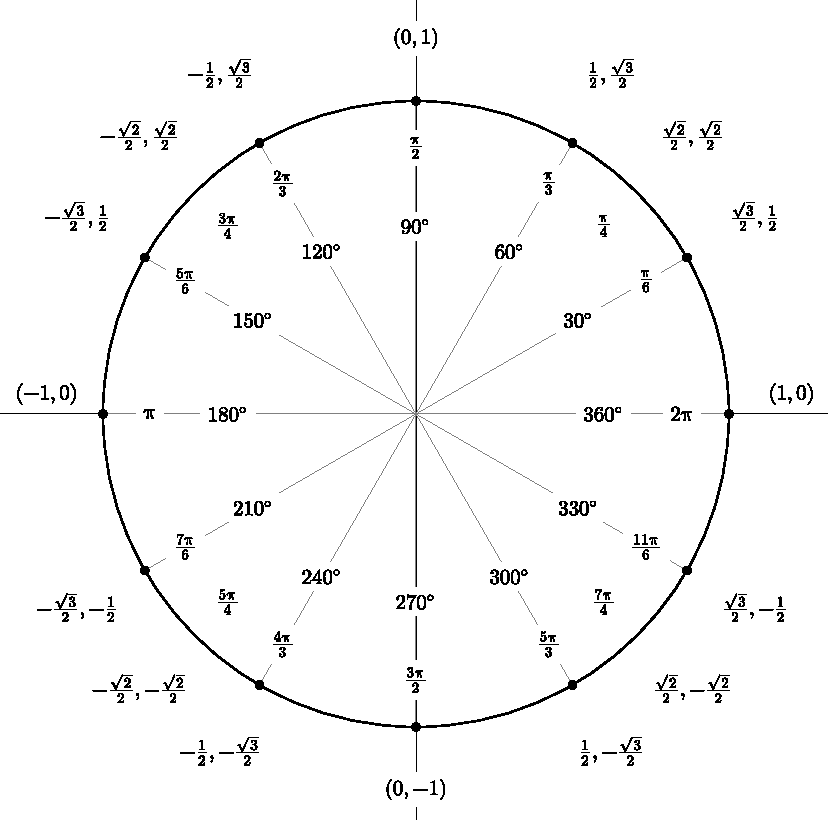
\includegraphics[width=0.7 \linewidth]{include_degrees_circle.pdf}
\end{center}

\begin{mainbox}{}
	\begin{center}
		\begin{tabular}{c|cccccc}
			deg & 0° & 30°                  & 45°                  & 60°                  & 90°             & 180°  \\
			\midrule
			rad & 0  & $\frac{\pi}{6}$      & $\frac{\pi}{4}$      & $\frac{\pi}{3}$      & $\frac{\pi}{2}$ & $\pi$ \\
			cos & 1  & $\frac{\sqrt{3}}{2}$ & $\frac{\sqrt{2}}{2}$ & $\frac{1}{2}$        & 0               & -1    \\
			sin & 0  & $\frac{1}{2}$        & $\frac{\sqrt{2}}{2}$ & $\frac{\sqrt{3}}{2}$ & 1               & 0     \\
			tan & 0  & $\frac{1}{\sqrt{3}}$ & 1                    & $\sqrt{3}$           & $+\infty$       & 0     \\
		\end{tabular}
	\end{center}
\end{mainbox}

\section{Analysis}

Sei \(\varphi : X \mapsto Y\) eine stetige Abbildung, wobei \(X=  X_0 \cup \partial X, \) \(Y = Y_0 \cup \partial Y\) kompakte Mengen mit \(X_0, Y_0\) offen und \(\partial X, \partial Y\) Nullmengen sind. Sei $\varphi$ ausserdem von $X_0$ nach $Y_0$ bijektiv und $C^1$. $J_\varphi(x)$ ist alle für alle $x \in X_0$ invertierbar.

\begin{subbox}{Variablenwechsel}
	$$\int_X f(\varphi(x)) | \det(J_\varphi(x)) | dx = \int_Y f(y) dy$$
\end{subbox}

\subsection{Potenzreihen}
\begin{align*}
	\exp(x)         & = \sumn \frac{x^n}{n!} = 1 + x + \frac{x^2}{2!} + \frac{x^3}{3!} + \cdots                  & r & = \infty \\
	\sin(x)         & = \sumn (-1)^n \frac{x^{2n + 1}}{(2n + 1)!} = x - \frac{x^3}{3!} + \frac{x^5}{5!} - \cdots & r & = \infty \\
	\cos(x)         & = \sumn (-1)^n \frac{x^{2n}}{(2n)!} = 1 - \frac{x^2}{2!} + \frac{x^4}{4!} - \cdots         & r & = \infty \\
	\ln(x + 1)      & = \sumk (-1)^{k+1} \frac{x^k}{k} = x - \frac{x^2}{2} + \frac{x^3}{3} - \cdots              & r & = 1      \\
	\sinh(x)        & = \sumn \frac{x^{2n+1}}{(2n+1)!} = x + \frac{x^3}{3!} + \frac{x^5}{5!} + \cdots            & r & = \infty \\
	\cosh(x)        & = \sumn \frac{x^{2n}}{(2n)!} = 1 + \frac{x^2}{2!} + \frac{x^4}{4!} + \cdots                & r & = \infty \\
	\arctan(x)      & = \sumn (-1)^n \frac{x^{2n+1}}{2n+1} = x - \frac{x^3}{3} + \frac{x^5}{5} - \cdots =        & r & = 1      \\
	e^{-x}          & = \sumn (-1)^n \cdot \frac{x^n}{n!} = 1 - x + \frac{x^2}{2!} - \frac{x^3}{3!} + \cdots     & r & = \infty \\
	\sqrt{1+x}      & = 1 + \frac{x}{2} - \frac{x^2}{8} + \frac{x^3}{16} + \mathcal{O}(x^4)                      & r & < 1      \\
	\frac{1}{1 - x} & = \sumn x^n                                                                                & x & < 1      \\
\end{align*}

\begin{mainbox}{Partielle Integration}
	$$\int f'(x) g(x) \mathop{dx} = f(x)g(x) - \int f(x) g'(x) \mathop{dx}$$
\end{mainbox}

\begin{itemize}
	\item Meist gilt: Polynome ableiten ($g(x)$), wo das Integral periodisch ist ($\sin, \cos, e^x$,...) integrieren ($f'(x)$)
	\item Teils: mit $1$ multiplizieren, um partielle Integration anwenden zu können (z.B. im Fall von $\int \log(x) \mathop{dx}$)
\end{itemize}

\textbf{Beispiel}: Berechne $\int x^2 \cos(x) dx = x^2 (-\frac{1}{3}\cos(3x)) - $

$2x(-\frac{1}{9}\sin(3x)) + 2\frac{1}{27}\cos(3x) - \int 0 \cdot \frac{1}{27} \cos(3x) dx$.

Multipliziere Diagonal wie im Beispiel.

\begin{table}[h]
	\begin{tabular}{lll}
		  & D     & I                      \\
		+ & $x^2$ & $\sin(3x)$             \\
		- & $2x$  & $-\frac{1}{3}\cos(3x)$ \\
		+ & $2$   & $-\frac{1}{9}\sin(3x)$ \\
		- & $0$   & $\frac{1}{27}\cos(3x)$
	\end{tabular}
\end{table}

Aufhören falls:
\begin{itemize}
	\item $0$ in D-Spalte.
	\item Produkt einer Reihe einfach integrierbar. Addiere oder subtrahiere je nach Reihe das Integral des Produkts.
	\item Eine Reihe wiederholt sich. Verwende Rekurrenz.
\end{itemize}

\begin{mainbox}{Substitution}
	Sei $g: [a, b] \to \mathbb{R}$ stetig differenzierbar. $f: I \to \mathbb{R}$ ($g([a, b]) \subseteq I$) eine stetige Funktion. Dann gilt:
	$$\int_{g(a)}^{g(b)} f(x)dx = \int_{a}^{b} f(g(x))g'(x)dt$$
\end{mainbox}

\begin{itemize}
	\item Grenzen substituieren nicht vergessen.
	\item Alternativ kann auch das unbestimmte Integral berechnet werden und dann $u$ wieder durch $x$ substituiert werden.
\end{itemize}

\begin{subbox}{Gamma-Funktion}
	Die Gamma-Funktion ist definiert als:
	$$\Gamma(s) := \int_0^\infty e^{-x}x^{s-1} dx = (s-1)!$$
	\begin{rowlist}
		\item $\Gamma(1) = 1$
		\item $\Gamma(\frac{1}{2}) = \sqrt{\pi}$
		\item $\Gamma(s + 1) = s \Gamma(s)$
	\end{rowlist}
\end{subbox}

Die regularisierte Gamma-Funktion ist definiert als $P(a, x) = \frac{\gamma(a, x)}{\Gamma(a)}$ wobei $\gamma(a, x) = \int_0^x t^{a - 1} e^{-t} dt$ und $\Gamma(a)$ wie oben.

\begin{mainbox}{Cauchy-Produkt}
	Das Cauchy-Produkt von zwei Reihen $\sum_{i = 0}^\infty a_i$ und $\sum_{j = 0}^\infty b_j$ ist definiert als
	$$\sum_{n=0}^\infty \sum_{j=0}^n (a_{n-j} \cdot b_j) = a_0b_0 + (a_0b_1 + a_1b_0) + \ldots$$ Es konvergiert, falls beide Reihen absolut konvergieren. Dann gilt:\\
	$$\sum_{n=0}^\infty \sum_{j=0}^n (a_{n-j} \cdot b_j) = \left( \sum_{i=0}^\infty a_i \right) \left( \sum_{j=0}^\infty b_j \right)$$
\end{mainbox}

\begin{mainbox}{Partialbruchzerlegung}
	Seien $p(x), q(x)$ zwei Polynome. $\int \frac{p(x)}{q(x)}$ wird wie folgend berechnet:
	\begin{enumerate}
		\item Falls $\deg(p) \ge \deg(q)$, führe eine Polynomdivision durch. Dies führt zum Integral $\int a(x) + \frac{r(x)}{q(x)}$.
		\item Berechne die Nullstellen von $q(x)$.
		\item Pro Nullstelle: Einen Partialbruch erstellen.
		      \begin{itemize}[left=0pt]
			      \item Einfach, reell: $x_1 \to \frac{A}{x - x_1}$
			      \item $n$-fach, reell: $x_1 \to \frac{A_1}{x - x_1} + \ldots + \frac{A_r}{(x-x_1)^r}$
			      \item Einfach, komplex: $x^2 + px + q \to \frac{Ax + B} {x^2 + px + q}$
			      \item $n$-fach, komplex: $x^2 + px + q \to \frac{A_1x+b_1}{x^2+px+q} + \ldots$
		      \end{itemize}
		\item Parameter $A_1, \ldots, A_n$ (bzw. $B_1, \ldots, B_n$) bestimmen. ($x$ jeweils gleich Nullstelle setzen, umformen und lösen).

	\end{enumerate}
\end{mainbox}

Für ein monisches Polynom $x^n + a_{n-1} x^{n-1} + \cdots + a_0 = 0$ muss jede Nullstelle $a_0$ teilen.\\

Häufig verwendete Partialbruchzerlegungen sind bspw. $\frac{1}{q(q+1)} = \frac{1}{q} - \frac{1}{q + 1}$ oder $\frac{1}{q(q-1)(q+1)} = \frac{-1}{q} + \frac{1}{2(q+1)} + \frac{1}{2(q-1)}$.

\subsection{Synthetische Division}
Berechne $\frac{6x^3 + 5x^2 - 7}{3x^2 - 2x - 1} = 2x + 3 + \frac{8x - 4}{3x^2 -2x - 1}$:\\
\begin{center}
	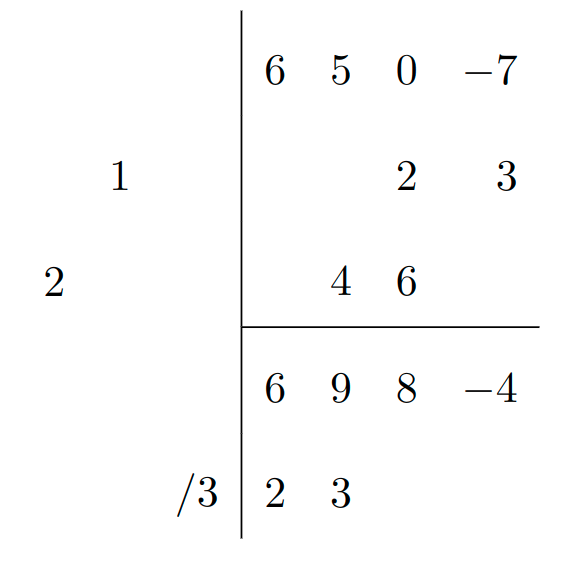
\includegraphics[width=0.4 \linewidth]{synthetic-division.png}
\end{center}

\subsection{Gerade und ungerade Funktionen}
\begin{itemize}
	\item Die Verknüpfung von ungeraden Funktionen ist ungerade.
	\item Sei $g$ gerade und $f$ beliebig. $f \circ g$ ist gerade.
	\item Sei $f$ gerade und $g$ ungerade. $g \circ f$ und $f \circ g$ sind gerade.
	\item Produkt einer geraden und einer ungeraden Funktion ist ungerade.
	\item Produkt zweier ungerader Funktionen ist gerade.
	\item Produkt zweier gerader Funktionen ist gerade.
	\item Für $f: [-a, a] \to \mathbb{R}$ stetig und ungerade, d.h. $f(-x) = -f(x)$ gilt $\int_{-a}^a f(x) dx = 0$.
\end{itemize}

\subsection{Uneigentliche Integrale}
$$\int_1^\infty \frac{1}{x^\alpha} dx = \begin{cases}
		\text{divergiert, }  & \alpha \leq 1 \\
		\frac{1}{\alpha - 1} & \alpha > 1
	\end{cases}$$
$$\int_0^1 \frac{1}{x^\alpha} dx = \begin{cases}
		\text{divergiert, } & \alpha \geq 1 \\
		\frac{1}{1- \alpha} & \alpha < 1
	\end{cases}$$
$$\int_0^\infty e^{-x} dx = 1$$
$$\int_0^\infty e^{-x}x^{s-1} dx = \begin{cases}
		\text{divergiert, } & s \leq 0 \\
		(s-1)!              & s > 0
	\end{cases}$$
$$\int_0^\infty \sin(x^2) dx = \sqrt{\frac{\pi}{8}}$$

\subsection{Binomischer Lehrsatz}

$$(x+y)^n = \sum_{k=0}^n {n \choose k} x^{n-k} y^k$$

\section{Tabellen}

\subsection{Grenzwerte}

\begin{center}
	\begin{tabularx}{\linewidth}{XX}
		\toprule
		$\limxi \frac{e^x}{x^m} = \infty$                          & $\limxn xe^x = 0$                        \\
		$\limxi (1+x)^{\frac{1}{x}} = 1$                           & $\limxo (1+x)^{\frac{1}{x}} = e$         \\
		$\limxi (1+\frac{1}{x})^b = 1$                             & $\limxi n^{\frac{1}{n}} = 1$             \\
		$\limxo \frac{e^x-1}{x} = 1$                               & $\limxi (1-\frac{1}{x})^x = \frac{1}{e}$ \\
		$\lim_{x\to\pm\infty} (1 + \frac{k}{x})^{mx} = e^{km}$     & $\limxi (\frac{x}{x+k})^x = e^{-k}$      \\
		$\limxo \frac{\log 1 - x}{x} = -1$                         & $\limxo x \log x = 0$                    \\
		$\limxo \frac{e^{ax}-1}{x} = a$                            & $\limxo \frac{\ln(x+1)}{x} = 1$          \\
		$\lim_{x\to 1} \frac{\ln(x)}{x-1} = 1$                     & $\limxi \frac{\log(x)}{x^a} = 0$         \\
		$\limxo \frac{a^x -1}{x} = \ln(a), \newline \forall a > 0$ &
		$\limxi x^a q^x = 0, \newline \forall 0 \le q < 1$                                                    \\
		$\limxo \frac{\sin x}{x} = 1$                              & $\limxo \frac{\sin kx}{x} = k$           \\
		$\limxo \frac{1}{\cos x} = 1$                              & $\limxo \frac{\cos x -1}{x} = 0$         \\
		$\limxo x \sin(\frac{1}{x}) = 0$                           & $\limxo x \log x = 0$                    \\
		$\limxo \frac{1 - \cos x}{x^2} = \frac{1}{2}$              & $\limxo \frac{e^x-1}{x} = 1$             \\
		$\limxo \frac{x}{\arctan x} = 1$                           & $\limxi \arctan x = \frac{\pi}{2}$       \\
		$\limxo \frac{e^{ax}-1}{x} = a$                            & $\limxo \frac{\ln(x+1)}{x} = 1$          \\
		$\lim_{x\to 1} \frac{\ln(x)}{x-1} = 1$                     & $\limxi \sqrt{x^2 + c} - x = 0$          \\
		$\limxi \sqrt[x]{x} = 1$                                   & $\limxi x(\sqrt[x]{n} - 1) = \ln(n)$     \\
		\bottomrule
	\end{tabularx}
\end{center}

\subsection{Ableitungen}

\begin{center}
	% the c>{\centering\arraybackslash}X is a workaround to have a column fill up all space and still be centered
	\begin{tabularx}{\linewidth}{c>{\centering\arraybackslash}Xc}
		\toprule
		$\mathbf{F(x)}$                        & $\mathbf{f(x)}$          & $\mathbf{f'(x)}$         \\
		\midrule
		$\frac{x^{-a+1}}{-a+1}$                & $\frac{1}{x^a}$          & $\frac{a}{x^{a+1}}$      \\
		$\frac{x^{a+1}}{a+1}$                  & $x^a \ (a \ne 1)$        & $a \cdot x^{a-1}$        \\
		$\frac{1}{k \ln(a)}a^{kx}$             & $a^{kx}$                 & $ka^{kx} \ln(a)$         \\
		$\ln |x|$                              & $\frac{1}{x}$            & $-\frac{1}{x^2}$         \\
		$\frac{2}{3}x^{3/2}$                   & $\sqrt{x}$               & $\frac{1}{2\sqrt{x}}$    \\
		$-\cos(x)$                             & $\sin(x)$                & $\cos(x)$                \\
		$\sin(x)$                              & $\cos(x)$                & $-\sin(x)$               \\
		$\frac{1}{2}(x-\frac{1}{2}\sin(2x))$   & $\sin^2(x)$              & $2 \sin(x)\cos(x)$       \\
		$\frac{1}{2}(x + \frac{1}{2}\sin(2x))$ & $\cos^2(x)$              & $-2\sin(x)\cos(x)$       \\
		\multirow{2}*{$-\ln|\cos(x)|$}         & \multirow{2}*{$\tan(x)$} & $\frac{1}{\cos^2(x)}$    \\
		                                       &                          & $1 + \tan^2(x)$          \\
		$\cosh(x)$                             & $\sinh(x)$               & $\cosh(x)$               \\
		$\log(\cosh(x))$                       & $\tanh(x)$               & $\frac{1}{\cosh^2(x)}$   \\
		$\ln | \sin(x)|$                       & $\cot(x)$                & $-\frac{1}{\sin^2(x)}$   \\
		$\frac{1}{c} \cdot e^{cx}$             & $e^{cx}$                 & $c \cdot e^{cx}$         \\
		$x(\ln |x| - 1)$                       & $\ln |x|$                & $\frac{1}{x}$            \\
		$\frac{1}{2}(\ln(x))^2$                & $\frac{\ln(x)}{x}$       & $\frac{1 - \ln(x)}{x^2}$ \\
		$\frac{x}{\ln(a)} (\ln|x| -1)$         & $\log_a |x|$             & $\frac{1}{\ln(a)x}$      \\
		\bottomrule
	\end{tabularx}
\end{center}


\subsection{Integrale}
\begin{center}
	\begin{tabularx}{\linewidth}{>{\centering\arraybackslash}X>{\centering\arraybackslash}X}
		\toprule
		$\mathbf{f(x)}$                     & $\mathbf{F(x)}$                                                     \\
		\midrule
		$\int f'(x) f(x) dx$                & $\frac{1}{2}(f(x))^2$                                               \\
		$\int \frac{f'(x)}{f(x)} dx$        & $\ln|f(x)|$                                                         \\
		$\int_{-\infty}^\infty e^{-x^2} dx$ & $\sqrt{\pi}$                                                        \\
		$\int (ax+b)^n dx$                  & $\frac{1}{a(n+1)}(ax+b)^{n+1}$                                      \\
		$\int x(ax+b)^n dx$                 & $\frac{(ax+b)^{n+2}}{(n+2)a^2} - \frac{b(ax+b)^{n+1}}{(n+1)a^2}$    \\
		$\int (ax^p+b)^n x^{p-1} dx$        & $\frac{(ax^p+b)^{n+1}}{ap(n+1)}$                                    \\
		$\int (ax^p + b)^{-1} x^{p-1} dx$   & $\frac{1}{ap} \ln |ax^p + b|$                                       \\
		$\int \frac{ax+b}{cx+d} dx$         & $\frac{ax}{c} - \frac{ad-bc}{c^2} \ln |cx +d|$                      \\
		$\int \frac{1}{x^2+a^2} dx$         & $\frac{1}{a} \arctan \frac{x}{a}$                                   \\
		$\int \frac{1}{x^2 - a^2} dx$       & $\frac{1}{2a} \ln\left| \frac{x-a}{x+a} \right|$                    \\
		$\int \sqrt{a^2 - x^2} dx $         & $\frac{a^2}{2} \arcsin(\frac{x}{a}) + \frac{x}{2} \sqrt{a^2 - x^2}$ \\
		$\int \csc(x) dx $                  & $\ln|\csc(x) + \cot(x)|$                                            \\
		$\int \sec(x) dx $                  & $\ln|\sec(x) + \tan(x)|$                                            \\
		$\int \cot(x) dx $                  & $\ln|\sin(x)|$                                                      \\
		$\frac{1}{\sqrt{1 - x^2}}$          & $\arcsin(x)$                                                        \\
		$\frac{-1}{\sqrt{1 - x^2}}$         & $\arccos(x)$                                                        \\
		$\frac{1}{1 + x^2}$                 & $\arctan(x)$                                                        \\
		$\frac{1}{\sqrt{1 + x^2}}$          & $\text{arsinh}(x)$                                                  \\
		$\frac{1}{\sqrt{x^2 - 1}}$          & $\text{arcosh}(x)$                                                  \\
		$\frac{1}{1 - x^2}$                 & $\text{artanh}(x)$                                                  \\
		$-\frac{1}{1 + x^2}$                & $\text{arccot}(x)$                                                  \\
		$x^x \cdot (1 + \ln x)$             & $x^x \ (x > 0)$                                                     \\
		$\sinh(x)$                          & $\cosh(x)$                                                          \\
		$\cosh(x)$                          & $\sinh(x)$                                                          \\
		\bottomrule
	\end{tabularx}
\end{center}

\clearpage
\newpage

\renewcommand*{\arraystretch}{2.5}
\begin{center}
	\small
	\begin{tabularx}{\textwidth}{llXXXXX}
		\toprule
		\textbf{Diskrete Verteilung} & Parameter                                       & \( \E[X] \) & \( \Var[X] \)       & \( p_X(t) \)         & \( F_X(t) \)                     & Eigenschaften \\
		\midrule
		Gleichverteilung    & \makecell[l]{\( n \): Anzahl Ereignisse                                                                                                                       \\ \( x_i \): Ereignisse} & \( \frac{1}{n} \sum_{i=1}^{n} x_i \) & \( \frac{1}{n} \sum_{i=1}^{n} x_i^2 - \frac{1}{n^2} \left(\sum_{i=1}^{n} x_i \right)^2 \) & \( \frac{1}{n} \) & \( \frac{|\{k:x_k \leq t\}|}{n} \) \\

		Bernoulli           & \( p: \) ErfolgsWK                              & \( p \)     & \( p \cdot (1-p) \) & \( p^t(1-p)^{1-t} \) & \( 1-p \) für \( 0 \leq t < 1 \)                 \\

		Binomial            & \makecell[l] {\( n \): Anzahl Versuche                                                                                                                        \\ \( p: \) ErfolgsWK } & \( np \) & \( np(1-p) \) & \( \binom{n}{t}p^t(1-p)^{n-t} \) & \( \sum_{k=0}^{t} \binom{n}{k} p^k(1-p)^{n-k} \)  \\

		Geometrisch         & \makecell[l] { \( p \): ErfolgsWK                                                                                                                             \\ \( t: \) Anzahl Versuche} & \( \frac{1}{p} \) & \( \frac{1-p}{p^2} \) & \( p(1-p)^{t-1} \) & \( 1-(1-p)^t\) & \begin{rowlist}
			\item gedächtnislos, $\P[X > t + s \mid X > s] = \P[X > t]$
		\end{rowlist} \\

		Poisson             & \makecell[l]{ \( \lambda > 0 \): Erwartungswert                                                                                                               \\ und Varianz} & \( \lambda \) & \( \lambda \) & \( \frac{\lambda^t}{t!}e^{-\lambda} \) & \( e^{-\lambda} \sum_{k=0}^{t} \frac{\lambda^{k}}{k!} \) &  \\

		Negativ-Binomial &  \makecell[l]{\( r: \) Anzahl Erfolge \\ \( p: \) ErfolgsWK} & $\frac{r(1-p)}{p}$ & $\frac{r(1-p)}{p^2}$ & ${t - 1 \choose r - 1} p^r (1-p)^{t - r}$ & I'd rather not \\

		\bottomrule
	\end{tabularx}
\end{center}

\begin{center}
	\small
	\begin{tabularx}{\textwidth}{llXXXXXX}
		\toprule
		\textbf{Stetige Verteilung}       & Parameter                      & \( \E[X] \)                                                             & \( \Var[X] \)                                                                                               & \( f_X(t) \)                                                                                                                                  & \( F_X(t) \)                                                                           & Eigenschaften                                                                                                          \\

		\midrule
		Gleichverteilung         & \( [a,b] \): Intervall         & \( \frac{a+b}{2} \)                                                     & \( \frac{1}{12}(b-a)^2 \)                                                                                   & \(\begin{cases} \frac{1}{b-a} &a \le t \le b \\ 0 & \text{sonst}\end{cases}\)                                                                 & \(\begin{cases} 0 & t\le a \\ \frac{t-a}{b-a} & a < t < b \\ 1 & t \ge b \end{cases}\)                                                                                                                          \\

		Exponentialverteilung    & \( \lambda: \frac{1}{\E[X]} \) & \( \frac{1}{\lambda} \)                                                 & \( \frac{1}{\lambda^2} \)                                                                                   & \( \begin{cases} \lambda e^{-\lambda t} & t \geq 0 \\ 0 & t < 0 \end{cases} \)                                                                & \( \begin{cases} 1-e^{-\lambda t} & t>0 \\ 0 & t \leq 0\end{cases}\)                   & \begin{rowlist}
			                                                                                                                                                                                                                                                                                                                                                                                                                                                                                             \item gedächtnislos, $\P[X > t + s \mid X > s] = \P[X > t]$
		                                                                                                                                                                                                                                                                                                                                                                                                                                                                                             \end{rowlist}                                                \\

		Normalverteilung         & \makecell[l]{\( \mu: \E[X] \)                                                                                                                                                                                                                                                                                                                                                                                                                                                                                                                                                            \\ \( \sigma^2 \): Varianz} & \( \mu \) & \( \sigma ^2 \) & \( \frac{1}{\sqrt{2\pi \sigma^2} }e^{-{\frac{(t-\mu)^2}{2\sigma^2} }} \) & \( \frac{1}{ {\sqrt{2\pi \sigma^2}}} \int_{-\infty}^t e^{-\frac{(y-\mu)^2}{2\sigma^2}} \mathrm{d} y \) \\

		\( \chi ^2 \)-Verteilung & \( n \): Freiheitsgrad         & \( n \)                                                                 & \( 2n \)                                                                                                    & \( \frac{1}{2^{\frac{n}{2}}\Gamma (\frac{n}{2})} t^{\frac{n}{2}-1} e^{-\frac{t}{2}} \text{ für } t>0\)                                        & \(P\left( \frac{n}{2}, \frac{t}{2}\right)  \)                                          & \begin{rowlist}
			                                                                                                                                                                                                                                                                                                                                                                                                                                                                                             \item Für $X_1, X_k$ unabhängig und standardnormalverteilt ist $Q := \sum_{i=1}^k X_i^2$ $\chi_k^2$-verteilt
			                                                                                                                                                                                                                                                                                                                                                                                                                                                                                             \item Ist $X \sim \chi_n^2$ dann ist $X \sim \gamma(\frac{n}{2}, \frac{1}{2})$
		                                                                                                                                                                                                                                                                                                                                                                                                                                                                                             \end{rowlist} \\

		t-Verteilung             & \( n \): Freiheitsgrad         & \( \begin{cases} 0 & n>1 \\ \text{undef.} & \text{sonst} \end{cases} \) & \( \begin{cases} \frac{n}{n-2} & n> 2 \\ \infty & 1<n \leq 2 \\ \text{undef.} & \text{sonst} \end{cases} \) & \( \frac{\Gamma \left( \frac{n+1}{2} \right) }{\sqrt{n\pi } \cdot \Gamma (\frac{n}{2})} \left( 1+ \frac{t^2}{n} \right) ^{- \frac{n+1}{2}} \) & I'd rather not                                                                         & \begin{rowlist}
			                                                                                                                                                                                                                                                                                                                                                                                                                                                                                             \item $\frac{\mathcal{N}(0,1)}{\sqrt{\frac{\chi_n^2}{n}}}$ ist t-verteilt mit $n$ Freiheitsgraden
			                                                                                                                                                                                                                                                                                                                                                                                                                                                                                             \item für $n = 1$ Cauchy
			                                                                                                                                                                                                                                                                                                                                                                                                                                                                                             \item für $n \to \infty$ Normal
		                                                                                                                                                                                                                                                                                                                                                                                                                                                                                             \end{rowlist}                                                  \\

		Cauchy                   & \makecell[l]{\( s > 0 \)                                                                                                                                                                                                                                                                                                                                                                                                                                                                                                                                                                 \\ \( -\infty < u < \infty \)} & - & - & $\frac{1}{\pi} \frac{s}{s^2 + (t - u)^2}$ & $\frac{1}{2} + \frac{1}{\pi} \arctan \left( \frac{t - u}{s} \right)$ & \begin{rowlist}
			\item symmetrisch zu $u$
		\end{rowlist} \\

		Gamma                    & \makecell[l]{\( p \)                                                                                                                                                                                                                                                                                                                                                                                                                                                                                                                                                                     \\ \( b \)} & $\frac{p}{b}$ & $\frac{p}{b^2}$ & $\begin{cases}
				\frac{b^p}{\Gamma(p)} t^{p - 1} e^{-bt} & t > 0    \\
				0                                       & t \leq 0
			\end{cases}$ & $\begin{cases}
				P(p, bt) & x \geq 0 \\
				0        & x < 0
			\end{cases}$ & \begin{rowlist}
				\item Für $p = 1$ und $b = \lambda$ exponentialverteilt ($\text{Exp}(\lambda)$)
				\item Die Summe von $n$ exponentialverteilten ZV ($\text{Exp}(\lambda)$) ist gamma-verteilt mit $p = n, b = \lambda$.
			\end{rowlist} \\

		\bottomrule
	\end{tabularx}
\end{center}

\end{document}